\documentclass[letterpaper]{article}
\usepackage{natbib,alifeconf}

\title{Developmental Embodied Agents as Meta-brain Models}
\author{Bradly Alicea$^{1}$, Stefan Dvoretskii$^{2}$, Sam Felder$^{3}$, Ziyi Gong$^{4}$, Ankit Gupta$^{5}$, \and Jesse Parent$^1$ \\
\mbox{}\\ 
$^1$Orthogonal Research and Education Laboratory, Champaign-Urbana, IL   USA \\
$^2$Technical University of Munich,  Germany \\
$^3$San Francisco, CA  USA \\
$^4$University of Pittsburgh,  PA   USA \\
$^5$IIT Kharaghpur, India \\
bradly.alicea@outlook.com}

\begin{document}
\maketitle

\begin{abstract}
We present a framework for meta-brain models, or hybrid models that capture multiple aspects of developmental neurobiology and behavior. A developmentally-inspired embodied learning agent architecture is combined with a contextually-explicit representational layer to form a complex artificial nervous system. The architectural description is summarized in terms of morphological differentiation, context-handling, and generalized architectural features. In conclusion, we propose potential functional milestones that help further explicate the usefulness of our approach. 
\end{abstract}

\section{Introduction}
Building life-like architectures introduces a modeling challenge. On the one hand, it is parsimonious to create a minimal model \citep{[1]}. This produces a desired behavior according to extremely simplified mechanisms and metaphors \citep{[2]}. An opposing view is that maximal representation \citep{[3]} is the only way we can truly capture realistic phenomena. This approach requires the synthesis of data and mechanisms from many different parts of an organism's biology \citep{[4]}. We will propose a third path toward simulating intelligent behavior, a generalized hybrid architecture called \textit{meta-brain models}. Meta-brain models are abstractions that capture essential structural and functional features of biological nervous systems. Additionally, meta-brain models should be computationally and conceptually diverse, encompassing multiple attributes of the simulated biology in a biologically-inspired manner. These include but are not limited to: explicit developmental processes, layering of hybrid model components, the introduction of innate mechanisms, and distinguishing between degrees of representation.

\section{Embodied Developmental Hybrid Agents}
We propose that embodied developmental agents that can integrate context are the way forward. In \citep{[5]}, developmental Braitenberg Vehicles (dBVs) are used to build a nervous system and interact with its environment. Braitenberg Vehicles \citep{[6]} are embodied agents that utilize a neuronal network (consisting of a dBVs intermediate nodes) to transfer information between sensor and effector. The vehicle interacts explicitly with the environment, as well as exhibiting both internal regulation and spatial awareness. The developmental component is implemented through changes in neuronal network connectivity with respect to time. Yet the developmental aspects of dBVs are not limited to mere connectivity. More generally, connectionist models \citep{[7]} have been found suitable for representing developmental phenomena such as the nonlinear generation of sequential growth and critical periods of learning.

Despite their developmental aspect, dBVs are largely representation-free in that they do not make any assumptions about the external world. There are in fact innate aspects to this architecture that serve well as a basal component of the meta-brain architecture. In their non-developmental models, BVs tend to exhibit habits that reflect excitatory and inhibitory connections between sensors, intermediate nodes, and effectors \citep{[8]}. BVs can exhibit rudimentary behaviors identified as "happiness", "love", or "aggression", which are associated with static body plans. The behaviors are rudimentary because they are essentially the outcome of hard-wired configurations. Suppose we make these connections plastic, and thus change their configuration over time. Will this result in significant fluctuations in the observed emotional state? To minimize this, a second layer is required to control behavioral degeneration due to the developmental process, particularly one that enables a contextual representation of emotional states.

\subsection{Morphological Differentiation as Growth}
Before we discuss the second layer of context, we must first address how to implement growth of a representation. Growth can be characterized as a form of morphological differentiation in which structure and/or function can become increasingly diverse. In this case, growth reflects increasing the size of a network. Yet as mentioned earlier, the growth of a dBV neuronal network can diversify (or in some cases obscure) the expression of habits and other behaviors. 

The meta-brain architecture presented here involves implementing a technique for neuronal network growth in dBVs (Figure 1). Network growth proceeds through \textit{connectivity-activation encoding}, in which matrix \textit{W(i,j)} of potential connections between intermediate nodes expands (potential connections increased) over developmental time. Updating \textit{W(i,j)} is generally a discrete process. We have approached connectivity-activation encoding using two different techniques: Hebbian Learning and Genetic Algorithms \citep{[9]}. Hebbian Learning has been used to introduce a basic form of multisensory integration to the dBV, while genetic algorithms have been used to enforce developmental recombination of existing nodes.

\begin{figure}[!htb]
\begin{center}
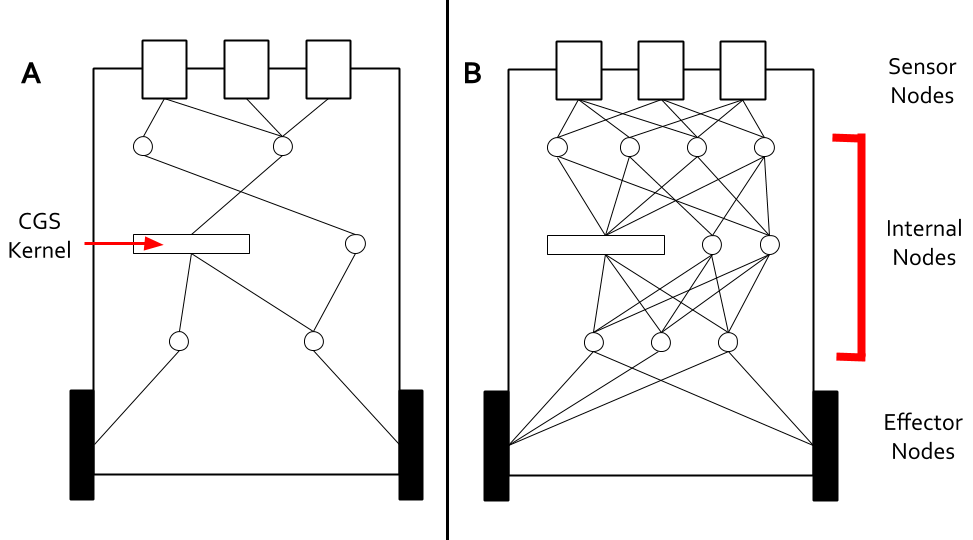
\includegraphics[width=2in]{Figure 1.png}
\caption{Figure 1. An example of wiring expansion in a hybrid dBV/CGS agent. A: earlier in the developmental process with fewer connections and the CGS embedded among the internal nodes. B: later in development after more redundant connections have emerged.}
\label{fig1}
\end{center}
\end{figure}

In the case of our Hebbian Learning approach, development is instantiated by building associations between between olfactory and gustatory stimuli, both distributed in a multidimensional space. The developmental process changes the connection weights in matrix \textit{W(i,j)} according to the co-occurrence of the two stimuli such that spatially-explicit multimodal associations can be acquired. Unfortunately, the Hebbian Learning approach is brittle and reveals a limited capacity for learning dynamically-changing spatial distributions of stimuli.

Our genetic algorithm generates a variety of topological orderings of matrix \textit{W(i,j)} through mutation and recombination. The fitness function that evaluates our dBVs neuronal network is based on stimulus-to-vehicle distance and force generated by vehicles in response to a given stimulus. Even though evolutionary variety randomizes matrix elements over time, selection nevertheless favors the emergence of specific behaviors such as spatial navigation. For larger dBV neuronal networks, we could use a Genetic Algorithm that encodes coordinated projection identity, which is similar to how axonogenesis proceeds in the \textit{Drosophila} nervous system \citep{[10]}.

\subsection{Morphological Differentiation as Layering}
The developmental process also includes a form of morphological differentiation called layering (Figure 2). Implementing a second layer as an extension of the first allows us to both benefit from the diversity of multiple models and better utilize the processing potential of layered neuronal structures. We utilize an representational approach called Contextual Geometric Structures (CGS), which allows us to capture multiple features of the environment as a surface bounded by overlapping dimensions \cite{[9]}. A soft classification scheme based on fuzzy logic is used to build representations with meaning and cultural significance. We can use phototaxis, or attraction/repulsion behaviors in response to light, as an example. While an unlayered dBV will simply exhibit a reactive behavior to light, a layered dBV coupled to a CGS will be able to evaluate the light source in the context of all physical gradations ranging from absolute light to absolute dark. 

\begin{figure}[!htb]
\begin{center}
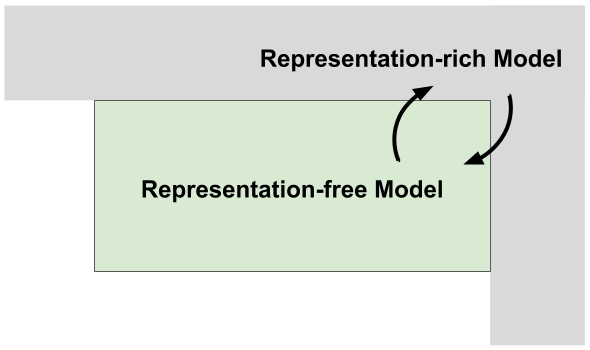
\includegraphics[width=2in]{Figure 2.png}
\caption{An example of generic layering in a sample agent.}
\label{fig2}
\end{center}
\end{figure}

CGS kernels create a binary opposition between two extreme labels, then use empirical data to build a model of the world. These empirical observations are made by the dBV, with connections between the intermediate nodes of the dBV and the CGS kernel. A CGS does not observe the world directly in this case, but operates on information processed by the dBV. When coupled with dBVs, CGS allow for stimuli for be mapped to a representational space that adds relational context to the original signal (Figure 2). This context then allows for greater control of outputs to the effector, as well as modulation of temporal changes in the dBV's neuronal network. 

\section{How to Develop Context}
Contextual behaviors emerge from interactions between the dBV architecture and the CGS classification kernel. Contextual behaviors are informed by long-term observations of the environment. Representation of such behaviors result from combining taxis and proportional membership in fuzzy categories (see Figure 3). We can take phototaxis as an example: dBVs will exhibit phototaxis, which are simple attraction/repulsion behaviors to a light stimulus. We can then use a one-dimensional CGS kernel to classify the relative presence or absence of light in the environment. The membership function over time will reflect the agent's experience with light (whether it is present or absent). In this way, we can incorporate not only probabilistic information, but higher-level interpretation of what the presence or absence of light means. 

Suppose we expand our representation to a two-dimensional kernel, with light-dark and safety-danger as the axes. We can establish lineages between observations of the presence of light and the result of being exposed to light (whether it is harmful or not). In this way, we combine associative learning introduced by a developing neuronal network in the dBV with conditional learning introduced by the CGS kernel. The action of both types of models can be combined without large amounts of data or a formal statistical distribution. While this does not prevent the agent from making category errors, it does provide a means to build \textit{nuance} from observations of the world using a common conceptual framework.

\begin{figure}[!htb]
\begin{center}
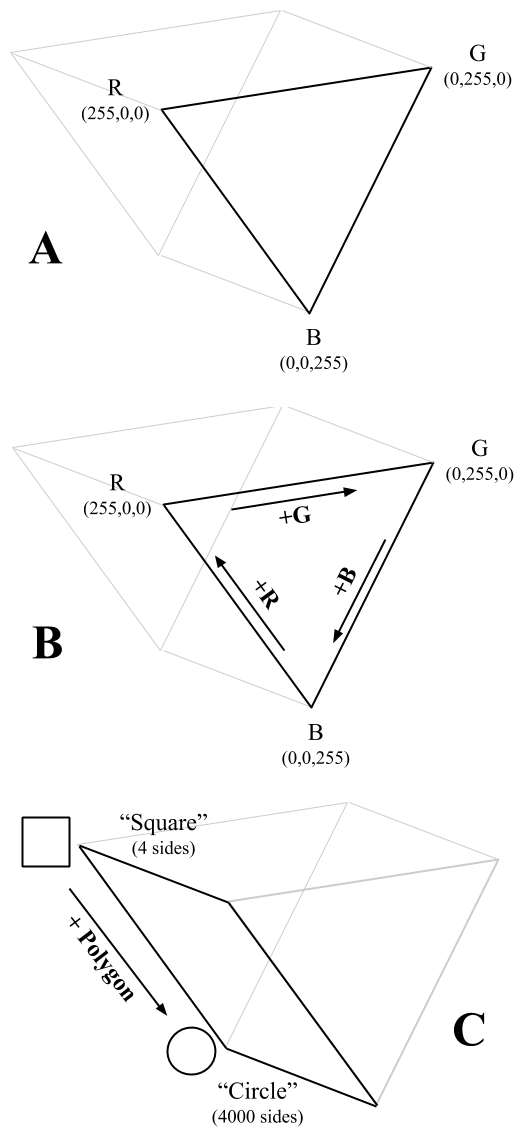
\includegraphics[width=2in]{Figure 3.png}
\caption{Membership functions for \textit{R,G,B,Polygon}. A and B represent the \textit{R,G,B} color space as CGS membership functions. C represents a related gradient of shape transformations (+ is increasing membership).}
\label{fig3}
\end{center}
\end{figure}

\section{Architectural Features}
We can potentially use a wide range of model types to introduce layering. Here, we use dBVs to process data from the environment along with CGS as a means to introduce representation of context. Using these two models in tandem creates both advantages and drawbacks. Any implementation of layering must allow for the following architectural features: innate components, dynamic components, and bio-inspired components.

\subsection{Innate Components}
In the implementation of contemporary neural networks, innateness is a forgotten but potentially crucial component in aiding the artificial learning process \citep{[11]}. Combining symbolic and connectionist architectures can draw upon the strengths of each type of formalism \citep{[12]}. Connectionist architectures are considered a form of sub-symbolic cognition, which can only approximate symbolic processes, and even then only under certain circumstances \citep{[13]}. Yet the dBV architecture is not the only innate aspect of our featured model. CGS kernels use basic concepts as innate components, often encoded as limits of a metric space.

In a traditional BV \citep{[6]}, simple behaviors are not so much learned as they are the product of excitation and inhibition of connections that link the sensors and effectors. The sensors take in information about the stimulus and transfer information towards the effector. This connection exists in either an excitatory or inhibitory state. This in turn controls movement of the vehicle's trajectory, which determines the behavioral state. We define vehicle trajectories in two ways \citep{[6]}: as a dot product (angle between two vectors) and as differential bilateral motion (continuous difference between left and right wheel rotation speeds). 

\subsection{Dynamic Components}
There are a number of ways to implement a dynamic set of processes that unfold over developmental time. These range from increasing numbers of neuronal cells to the cumulative effects of stimulus encounters and even the gradual interfacing between layers. The dBV-CGS is a tightly-coupled hybrid architecture \citep{[11]} in which an embodied lower layer is crucial. In general, embodiment is a critical component of animal development, as it enables learning and behavioral coordination \citep{[14]}.

One dynamic component is the relationship between the connectivity-activation encoding of a traditional BV and the more dynamic (and potentially unstable) connectivity-activation encoding of a dBV. We can revisit this not as something that needs to be dynamically regulated, but as something that can be used as a difference to be understood. This differential output is captured in terms of trajectory (as mentioned in the last section), and is fed to the CGS representational layer to enable contextual classification. 

\subsection{Bio-inspired Components}
We can also exploit the biological features of development to govern both the growth of neuronal networks within dBVs and the layering of dBVs and CGS components. For example, morphogenesis of the \textit{C. elegans} connectome is defined by three properties: most neuronal cells are born within a 135 minute window, conservation of cell spatial position from development to adulthood, and temporal separation of neuronal differentiation and electrical connectivity \citep{[15]}, \citep{[16]}. We can also build upon heterochronic mechanisms \citep{[17]}, \citep{[18]} to control system growth in a manner that invokes innateness. Of particular interest is the ability to simulate how different modules of the hybrid system develop at distinct rates.

\section{Discussion}
Now that we have demonstrated how a heterogeneous hybrid representation can simulate development and behavior \citep{[19]}, we must consider how a expansive and layered system might improve performance on a number of functional milestones. While we have not formally benchmarked our architecture on these tasks, they might serve as future goals for implementation.

One example of how a representation-rich architecture might improve the performance of a dBV is the ability to learn \textit{chromotaxis}. Chromotaxis are built from phototaxis exhibited by the dBV, but use a CGS representation of \textit{R,G,B} components of a light source to enable distinctions between different properties in the same source. While this requires color information and the appropriate CGS representation, it also allows for more nuanced behaviors to be exhibited by the dBV.

Multisensory integration is known for its nonlinear effects, particularly the sub- and super-additive effects of spatial coincidence \citep{[20]}. When multiple sensory components of a stimulus are presented in the same location, the response is superadditive. We have shown that this can be a mechanism of connectivity-activation encoding in dBVs. In future work, we will seek to understand multisensory integration as a function of the representational layer (CGS).

Lastly, the CGS representation allows membership functions of objects to be derived for multiple categories. For example, suppose all objects are aggression-provoking, cowardness-provoking, and love-provoking. A given stimulus is classified as 55 percent aggression-provoking, 30 percent cowardness-provoking, and 10 percent love-provoking. This refines object classification and can resolve ambiguous or novel intermediate behaviors.

\footnotesize
\bibliographystyle{apalike}
\bibliography{bibliography.bib}
\end{document}
